BE and CF are two equal altitudes of a triangle ABC.
\captionsetup{justification=centering}
\begin{figure}[!h]
\centering
\resizebox{\columnwidth}{!}{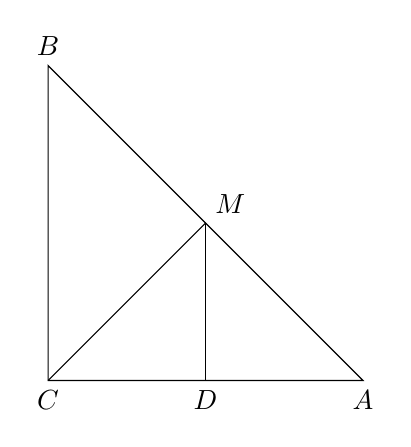
\begin{tikzpicture}
\coordinate (B) at (0,4);
\coordinate (A) at (4,0);
\coordinate (C) at (0,0);
\coordinate (D) at (2,0);
\coordinate (M) at (2,2);
\draw (A)node[below]{$A$}--(B)node[above]{$B$}--(C)node[below]{$C$}--cycle;
\draw(M)node[above right]{$M$}--(D)node[below]{$D$};
\draw(M)--(D);
\draw(M)--(C);
\tkzMarkRightAngle(B,C,A)
\tkzMarkRightAngle(A,D,M)
\tkzMarkRightAngle(C,D,M)
\end{tikzpicture}
}
\caption{Triangle with equal altitudes on two sides}
\label{eq:solutions/1/36/myfig}
\end{figure}
Given:-\\
1) Altitudes are Equal means their magnitude are same
 \begin{align}
 	\norm{\vec{E} - \vec{B}} = \norm{\vec{F} - \vec{C}} \label{eq:solutions/1/36/1}
 \end{align}
2) Altitude makes right angle at the base therefore $\cos 90 =0$ therefore  FC $\perp$ BF and EB $\perp$ CE where $\textbf{m}$ is the directional vectors.
\begin{align}
\textbf{m}_{FC} \textbf{m}_{BF} = 0 \label{eq:solutions/1/36/2}\\
\textbf{m}_{EB} \textbf{m}_{CE} = 0 \label{eq:solutions/1/36/3}
\end{align}
From \eqref{eq:solutions/1/36/2}
\begin{align}
    \brak{\vec{B}-\vec{F}}^T\brak{\vec{F}-\vec{C}}=\vec{0} && \brak{\vec{F}-\vec{C}}^T\brak{\vec{B}-\vec{F}}=\vec{0}\label{eq:solutions/1/36/4}
\end{align}
From \eqref{eq:solutions/1/36/2} and using \eqref{eq:solutions/1/36/4} 
\begin{align}
    \brak{\vec{B}-\vec{C}}^T\brak{\vec{B}-\vec{C}}\\
    =\brak{\vec{B}-\vec{F}+\vec{F}-\vec{C}}^T\brak{\vec{B}-\vec{F}+\vec{F}-\vec{C}})
    \end{align}
    \begin{align}
      =\brak{\vec{B}-\vec{F}}^T\brak{\vec{B}-\vec{F}}+\brak{\vec{F}-\vec{C}}^T\brak{\vec{F}-\vec{C}} 
    \end{align}
\begin{align}
   \norm{\vec{B}-\vec{C}}^2=\norm{\vec{B}-\vec{F}}^2+\norm{\vec{F}-\vec{C}}^2\label{eq:solutions/1/36/8} 
    \end{align}
    Similarly\\
    From \eqref{eq:solutions/1/36/3}
    \begin{align}
        \brak{\vec{E}-\vec{B}}^T\brak{\vec{E}-\vec{C}}=\vec{0} && \brak{\vec{E}-\vec{C}}^T\brak{\vec{B}-\vec{E}}=\vec{0}\label{eq:solutions/1/36/9}
        \end{align}
From  \eqref{eq:solutions/1/36/3} and using \eqref{eq:solutions/1/36/9}  
\begin{align}
    \brak{\vec{B}-\vec{C}}^T\brak{\vec{B}-\vec{C}}\\
    =\brak{\vec{B}-\vec{E}+\vec{E}-\vec{C}}^T\brak{\vec{B}-\vec{E}+\vec{E}-\vec{C}}
    \end{align}
    \begin{align}
      =\brak{\vec{B}-\vec{E}}^T\brak{\vec{B}-\vec{E}}+\brak{\vec{E}-\vec{C}}^T\brak{\vec{E}-\vec{C}} 
    \end{align}
\begin{align}
   \norm{\vec{B}-\vec{C}}^2=\norm{\vec{B}-\vec{E}}^2+\norm{\vec{E}-\vec{C}}^2\label{eq:solutions/1/36/13}
    \end{align}        
    Equating \eqref{eq:solutions/1/36/8} and \eqref{eq:solutions/1/36/13} and using \eqref{eq:solutions/1/36/1}
    \begin{align}
      \norm{\vec{B}-\vec{F}}^2+\norm{\vec{F}-\vec{C}}^2 = \norm{\vec{B}-\vec{E}}^2+\norm{\vec{E}-\vec{C}}^2  
    \end{align}
    \begin{align}
       \norm{\vec{B}-\vec{F}}^2=\norm{\vec{E}-\vec{C}}^2\\
       =\norm{\vec{B}-\vec{F}}=\norm{\vec{E}-\vec{C}}\label{eq:solutions/1/36/16}
    \end{align}
Let $\angle FBC=\theta_1$  and  $\angle EBC=\theta_2$
    \begin{align}
        \brak{\vec{B}-\vec{F}}^T\brak{\vec{B}-\vec{C}}=\norm{\vec{B}-\vec{F}}\norm{\vec{B}-\vec{C}}\cos\theta_1\\
        \cos{\theta_1}=\frac{\brak{\vec{B}-\vec{F}}^T\brak{\vec{B}-\vec{C}}}{\norm{\vec{B}-\vec{F}}\norm{\vec{B}-\vec{C}}}\\
        \cos{\theta_1}=\frac{\brak{\vec{B}-\vec{F}}^T\brak{\vec{B}-\vec{F}+\vec{F}-\vec{C}}}{\norm{\vec{B}-\vec{F}}\norm{\vec{B}-\vec{C}}}\\
        \cos{\theta_1}=\frac{\brak{\vec{B}-\vec{F}}^T\brak{\vec{B}-\vec{F}} +\brak{\vec{B}-\vec{F}}^T\brak{\vec{F}-\vec{C}}}{\norm{\vec{B}-\vec{F}}\norm{\vec{B}-\vec{C}}}
        \end{align}
        From \eqref{eq:solutions/1/36/4}
        \begin{align}
          \cos{\theta_1}=\frac{\brak{\vec{B}-\vec{F}}^T\brak{\vec{B}-\vec{F}}}{\norm{\vec{B}-\vec{F}}\norm{\vec{B}-\vec{C}}} \\
          \cos{\theta_1}=\frac{\norm{\vec{B}-\vec{F}}^2}{\norm{\vec{B}-\vec{F}}\norm{\vec{B}-\vec{C}}}\\
          \cos{\theta_1}=\frac{\norm{\vec{B}-\vec{F}}}{\norm{\vec{B}-\vec{C}}}
        \end{align}
        Similarly for $\angle EBC=\theta_2$
       \begin{align}
        \brak{\vec{C}-\vec{E}}^T\brak{\vec{B}-\vec{C}}=\norm{\vec{C}-\vec{E}}\norm{\vec{B}-\vec{C}}\cos\theta_2\\
        \cos{\theta_2}=\frac{\brak{\vec{C}-\vec{E}}^T\brak{\vec{B}-\vec{C}}}{\norm{\vec{C}-\vec{E}}\norm{\vec{B}-\vec{C}}}\\
        \cos{\theta_2}=\frac{\brak{\vec{C}-\vec{E}}^T\brak{\vec{B}-\vec{E}+\vec{E}-\vec{C}}}{\norm{\vec{C}-\vec{E}}\norm{\vec{B}-\vec{C}}}\\
        \cos{\theta_2}=\frac{\brak{\vec{C}-\vec{E}}^T\brak{\vec{B}-\vec{E}} +\brak{\vec{C}-\vec{E}}^T\brak{\vec{E}-\vec{C}}}{\norm{\vec{C}-\vec{E}}\norm{\vec{B}-\vec{C}}}
        \end{align}
        From {\eqref{eq:solutions/1/36/9}}
        \begin{align}
          \cos{\theta_2}=\frac{\brak{\vec{C}-\vec{E}}^T\brak{\vec{C}-\vec{E}}}{\norm{\vec{C}-\vec{E}}\norm{\vec{B}-\vec{C}}} \\
          \cos{\theta_2}=\frac{\norm{\vec{C}-\vec{E}}^2}{\norm{\vec{C}-\vec{E}}\norm{\vec{B}-\vec{C}}}\\
          \cos{\theta_2}=\frac{\norm{\vec{C}-\vec{E}}}{\norm{\vec{B}-\vec{C}}}
        \end{align}
        From \eqref{eq:solutions/1/36/16} we know $\norm{\vec{B}-\vec{F}}=\norm{\vec{E}-\vec{C}}$ we conclude
        \begin{align}
            \cos\theta_1=\cos\theta_2
            \implies\theta_1=\theta_2
        \end{align}
        So the sides opposite to equal angles are equal. Hence AB=AC hence the given Triangle is isosceles.
